\documentclass[12pt,a4paper,final]{report}
\usepackage[english]{babel}
\usepackage[fleqn]{amsmath}
\usepackage{amsfonts}
\usepackage{amssymb}
\usepackage{mathptmx}
\usepackage{fancyhdr}
\usepackage{graphicx}
\usepackage{array}

\usepackage[%
    a4paper,
%   includeheadfoot,
    head=0.762cm,  % distance from bottom of header to block of text aka \headsep e.g. \baselineskip
    foot=0.762cm,  % distance from top of footer to block of text aka \footskip
    headheight=12pt,     % height for the header block (no equivalent for footer)
%   heightrounded,       % ensure an integer number of lines
    marginparwidth=2cm,  % right marginal note width
    marginparsep=2mm,    % distance from text block to marginal note box
%   height=\textheight,  % height of the text block
%   width=\textwidth,    % width of the text block
    top=1.7cm,           % distance of the text block from the top of the page
    bottom=1.4cm,
    left=1.9cm,
    right=1.9cm,
%    showframe,           % show the main blocks
%    verbose,             % show the values of the parameters in the log file
]{geometry}

\pagestyle{fancy}
\fancyhf{}
\rhead{\bfseries {\nouppercase{\leftmark}}}
\lhead{\bfseries DDoS Detection in Software Defined Network}
\cfoot{\bfseries \thepage}

\usepackage[table]{xcolor}
\newcolumntype{P}[1]{>{\centering\arraybackslash}p{#1}}
\newcolumntype{M}[1]{>{\centering\arraybackslash}m{#1}}

\renewcommand{\footrulewidth}{0.4pt}

\title{Detection of DDoS in SDN environment using SVM and Entropy based discretization.}
\graphicspath{ {Images/} }

\usepackage{tikz}
\usetikzlibrary{calc}
\usepackage{eso-pic}

\usepackage{titlesec}
\titleformat{\section}[block]
  {\fontsize{16}{18}\bfseries}
  {\thesection}
  {1em}
  {}
\titleformat{\subsection}[block]
  {\fontsize{14}{15}\bfseries}
  {\thesubsection}
  {1em}
  {}

\usepackage{blindtext}
\usepackage{tocloft}
\renewcommand{\cfttoctitlefont}{\hspace*{\fill}\Huge\bfseries}
\renewcommand{\cftaftertoctitle}{\hspace*{\fill}}
\renewcommand{\cftlottitlefont}{\hspace*{\fill}\Huge\bfseries}
\renewcommand{\cftafterlottitle}{\hspace*{\fill}}
\renewcommand{\cftloftitlefont}{\hspace*{\fill}\Huge\bfseries}
\renewcommand{\cftafterloftitle}{\hspace*{\fill}}

\newcommand{\abbrlabel}[1]{\makebox[6cm][l]{\textbf{#1}\ \dotfill}}
\newenvironment{abbreviations}{\begin{list}{}{\renewcommand{\makelabel}{\abbrlabel}}}{\end{list}}

\DeclareRobustCommand{\gobblefive}[5]{}
\newcommand*{\SkipTocEntry}{\addtocontents{toc}{\gobblefive}}

\usepackage{hyperref}
\hypersetup{
    colorlinks=true,
    linkcolor=black,
    citecolor=black,
}

\begin{document}
\begin{center}
\thispagestyle{empty}
\vspace*{1cm}
A PRELIMINARY PROJECT REPORT
\vspace*{0.75cm}

ON
\vspace*{0.75cm}

\Large
DETECTION OF DDoS IN SDN ENVIRONMENT USING SVM AND ENTROPY  BASED DISCRETIZATION.
\vspace*{0.75cm}

\normalsize
\begin{figure}[h]
\begin{center}

\includegraphics[width=5.5cm, height=6cm]{logo.png}
\end{center}
\end{figure}

\vspace*{0.5cm}
BY
\vspace*{0.35cm}
\linebreak
ACHYUTH RAO
\linebreak
AKIB SHAIKH
\linebreak
ARUN POTTEKAT
\linebreak
PRANAV TALE
\linebreak

\large
\vspace*{0.5cm}
DEPARTMENT OF COMPUTER ENGINEERING
\linebreak
P.E.S MODERN COLLEGE OF ENGINEERING
\linebreak
PUNE - 411005.
\linebreak
$[$ 2016 – 2017 $]$
\end{center}
\newpage

\thispagestyle{empty}
\vspace*{60px}
\underline{\hspace{16cm}}
\vspace*{30px}

\begin{center}
\textbf{A PRELIMINARY PROJECT REPORT}\\

\vspace*{25px}
\textbf{ON}

\vspace*{25px}

\begin{huge}
\textbf{``Detection of DDoS in SDN Environment using SVM and Entropy based discretization''}\par
\end{huge}

\vspace*{13px}
\textbf{Version: 1.0, \today}

\vspace*{40px}
\textbf{By}\\

\vspace*{30px}
\textbf{Achyuth Rao}\\
\textbf{Akib Shaikh}\\
\textbf{Arun Pottekat}\\
\textbf{Pranav Tale}

\end{center}

\vspace*{5cm}
\underline{\hspace{16cm}}
\newpage

\thispagestyle{empty}
\vspace*{7cm}

\textbf{Guide:}

\begin{itemize}
\addtolength{\itemindent}{.5cm}
\item \textbf{Internal Guide Name:} Ms. Aparna Junnarkar

\end{itemize}

\vspace{1cm}

\textbf{Presented By:}

\begin{center}

\begin{tabular}{|>{\bf}m{3.5cm}|>{\bf}m{3.5cm}|>{\bf}m{3.5cm}|>{\bf}m{3.5cm}|}
\hline
\rowcolor{lightgray}
Date & Version & Title & Authors \\
\hline
\normalfont{$6^{th}$ October, 2016} & 
\normalfont{1.0} & 
\normalfont{Detection of DDoS in SDN Environment using SVM and Entropy based discretization} & 
\normalfont{Achyuth Rao, Akib Shaikh, Arun Pottekat, Pranav Tale}\\
\hline
\end{tabular}

\end{center}
\newpage

\thispagestyle{empty}
\vspace*{1.3cm}
\begin{center}

\includegraphics[width=5.5cm, height=6cm]{logo.png}
\end{center}
\begin{center}
\Large
Progressive Education Society's \\
\textbf{Modern College of Engineering} \\
Shivajinagar, Pune - 411005. \\
\vspace{1cm}

\underline{\textbf{CERTIFICATE}}
\end{center}
\normalsize
\vspace{0.5cm}
This is to certify that the following students of Final Year Computer Engineering have successfully completed the preliminary analysis and design of project entitled ``Detection of DDoS in SDN environment using SVM and Entropy based mechanism'' for the organization ``PES Modern College Of Engineering'' \\
The Group Members names are: \hspace{0.1cm} Sandhyavandanam Achyuth Rao. \\\hspace*{5.7cm} Akib Ashraf Shaikh. \\
\hspace*{5.7cm} Arun Pramod Pottekat. \\
\hspace*{5.7cm} Pranav Balasaheb Tale. \vspace{1cm}\\
This is in partial fulfillment of Bachelor of Computer Engineering under Savitribai Phule Pune University. \vspace{1cm}\\
Date: \vspace{2cm} \\
\hspace*{0.8cm}Internal Guide 	 
\hspace{3.95cm}Head Of Dept
\hspace{3.5cm}External Examiner \\
(Ms. Aparna Junnarkar)
\hspace*{2.3cm}(Computer Engineering) \\
\hspace*{6.3cm}(Dr. Prof. Mrs. S. A. Itkar) \\

\thispagestyle{empty}
\Large
\begin{center}
\chapter*{\centering Acknowledgement}
\end{center}
\normalsize
It gives us pleasure in presenting the preliminary project report on \textbf{`Detection of Distributed Denial of service attack in Software Defined Network using Support Vector Machine and Entropy Based Discretization'}.\\

Firstly, we would like to express our indebtedness appreciation to our internal guide \textbf{Ms. Aparna A. Junnarkar}. Her constant guidance and advice played very important role in making the execution of the report. She always gave us her suggestions, that were crucial in making this report as flawless as possible.\\

We would like to express our gratitude towards \textbf{Prof. Dr. Mrs. S. A. Itkar}  Head of Computer Engineering Department, PES Modern College of Engineering for her kind co-operation and encouragement which helped us during the completion of this report.\\

Also, we would like to thank \textbf{Mr. Kunal Khadke, Ms. Yogita Narwadkar, Mr. B. D. Phulpagare, Ms. Pallavi Baviskar, Ms. Deipali V. Gore, Ms. Renuka Kajale} and all \textbf{Technical assistants} for providing time to time guidance and various resources such as laboratory with all needed software platforms and continuous Internet connection for our Project.\\

In the end special thanks to all our classmates for helping us out during the entire documentation process.

\begin{flushright}
Achyuth Rao\\
Akib Shaikh\\
Arun Pottekat\\
Pranav Tale\\
\end{flushright}
\newpage

\pagestyle{plain} 
\cleardoublepage
\pagenumbering{gobble}
\tableofcontents
\newpage

\pagenumbering{roman}
\Large
\chapter*{\centering Abstract}
\addcontentsline{toc}{chapter}{Abstract}
\normalsize
\noindent
The current networking paradigm involves switches, routers and gateways where these networking devices constitute both logical thinking as well as routing of packets. Traditionally the network administrator is responsible for configuring and managing these devices manually and at all times, which makes it a tedious task. 

With the onset of the Software Defined Network, this task of manually managing the devices reduces to some extent, as it seperates the control plane from the data plane i.e. Forwarding of
packets is done in the data plane and intelligence of the entire network resides in the control plane. 

Data plane constitutes the network devices which comprise switches known as "dumb terminals" and the control plane constitutes a central controller which keeps track of all switches in the network.

Due to the centralized nature of SDN i.e. the controller at the center of SDN taking the logical decisions, there arises a threat of malicious users launching cyber attacks on this central component thereby, dislodging the entire network. Some attacks include Application level attacks, Brute Force attack, man in the middle attacks, DDoS attack etc.

Distributed Denial of Service attack involves a single malicious user controlling different users known as bots to launch an attack
against a single entity in the network without even the victim being aware of the attack. DDoS attacks result in direct financial losses along with damage to company reputation and loss of the customer's trust.

As a part of solution to this problem, two algorithms can be used for the detection of DDoS attack i.e. Support Vector Machine, a machine learning algorithm and Entropy based Discretization, a Data Mining algorithm.

Support Vector Machine takes the rate of incoming packets as the input and classifies them as normal traffic or attack traffic. Whereas Entropy based Discretization monitors the entropy of the network i.e. measure of randomness and if it falls below a threshold value then it is classified as attack traffic.

Once the attack is detected by either of the applications, an entry will be made in the log files  constantly monitored by network monitoring tools and thus report the incident back to the network adminstrative team. 

The network adminstrator would be provided a monitoring application which would display the details of the attack detected such as the source IP and victim IP etc.

As a part of the project, comparison studies will also be done related to both algorithms displaying the rate at which attacks are detected along with their accuracies.
\newpage

\listoffigures
\addcontentsline{toc}{chapter}{List of Figures}
\newpage
\listoftables
\addcontentsline{toc}{chapter}{List of Tables}
\newpage

\chapter*{\centering List of Abbreviations}
\begin{abbreviations}
\item[SDN] Software Defined Network
\item[SVM] Support Vector Machine
\item[DDoS] Distributed Denial of Service
\item[ONOS] Open Network Operating Switch
\item[OVSDB] Open vSwitch Database
\item[EBD] Entropy based Discretization
\item[NP] Non Polynomial Time
\item[P] Polynomial Time
\item[HTTP] Hyper Text Transfer Protocol
\item[UDP] Uniform Datagram Protocol
\item[TCP] Transmission Control Protocol
\item[k-NN] K Nearest Neighbour
\item[ICMP] Internet Control Message Protocol
\item[FTP] File Transfer Protocol
\item[QP] Quadratic problem
\end{abbreviations}

\addcontentsline{toc}{chapter}{List of Abbreviations}
\newpage
\pagestyle{fancy}
 
\newcommand{\hsp}{\hspace{0pt}}
\titleformat{\chapter}[hang]
{\flushright\fontseries{b}\fontsize{80}{100}\selectfont}{\fontseries{b}\fontsize{72}{84}\selectfont\textcolor{black}\thechapter\hsp}{0pt}
{.\\ \Huge\bfseries}
[]\titlespacing*{\chapter}{0pt}{540pt}{20pt}	

\pagenumbering{gobble}
\pagenumbering{arabic}

\AddToShipoutPictureBG*{%
\begin{tikzpicture}[overlay,remember picture]
\draw[line width=1.5pt]
    ($ (current page.north west) + (0.7cm,-0.7cm) $)
    rectangle
    ($ (current page.south east) + (-0.7cm,0.7cm) $);
\draw[line width=1.5pt]
    ($ (current page.north west) + (0.9cm,-0.9cm) $)
    rectangle
    ($ (current page.south east) + (-0.9cm,0.9cm) $);
\end{tikzpicture}
}
\chapter{Introduction}
\thispagestyle{empty}
\newpage
\section{Overview}
Software Defined Networking(SDN) is a promising approach that enables superior network control by providing the ability to change, manage and control, the behaviour of the network and the network devices in a dynamic manner. The separation of control plane (responsible for taking networking decisions) from the data plane (responsible for forwarding the packets) introduces programmability into the network. However this architecture brings to light many security issues.

SDN market is expected to reach 12.5 billion dollars by the year 2020. As the number of SDN deployments increase it becomes a necessity to solve these security issues and threats. A successful Distributed Denial of Service (DDoS) attack can make the resources unavailable and cripple the entire network.

This project combines the concepts of next-generation networking along with machine learning and data mining approaches in order to solve the security issues in SDN. Our aim is to detect the DDoS attack using either Support Vector Machine (SVM) classifier or Entropy Based Discretization and generate an alert so that later it can be effectively mitigated. The acceptance of a solution in an industry depends on its successful functioning in a real world scenario. The final solution will be such that it can actually be used in the SDN deployed environments. 

\section{Brief Description}
\begin{enumerate}
\item 
The intelligence of the network is logically centralized to a control unit called the controller, which has the knowledge of the complete network. Recent DDoS attacks are of the scale of 600 Gbit/s and are very effective in exhausting the resources of the controller.

\item
We propose and compare two solutions for detection of DDoS attack namely, Support Vector Machine classifier based on Machine Learning and Entropy-Based Discretization based on data mining.

\item
The SVM or Entropy application will be running on edge switches and by analyzing the continuously changing data of the flow table the attack will be detected.

\item
A network monitoring tool such as Nagios is used and configured such that as soon as the attack is detected an alert is generated and sent to the network administrator so that further steps can be taken for effectively mitigating the attack.
\end{enumerate}

\section{Problem Definition}
The next generation network i.e. Software Defined Network will be classified as a revolutionary step in the networking paradigm, owing to the seperation of control plane and data plane which results in better network management and increases throughput. However, such a change comes at a huge cost, wherein due to centralization of the entire network, there is a risk to the network from network attacks such as DDoS etc. Hence, we propose a solution for detection of one such network attack i.e. Distributed Denial of Service attack in a Software Defined Network using Support Vector Machine and Entropy based discretization algorithms.

\section{Project Objectives}
\begin{enumerate}
\item
Deploying a custom topology of Software Defned Network for experimentation in a virtual environment using a network simulation tool like Mininet and configuring Raspberry Pi's to function as OpenFlow switches.

\item
Training the SVM classifier to detect the attack using an environment-specific data set.

\item
Selecting the threshold value based on the environment traffic and comparing the calculated entropy with the threshold to detect the attack packets.

\item
Running the SVM or Entropy application on the edge switches so that the run-time data can be analyzed by extracting the flow table information from the switch and classifying or performing calculation to analyze the packets.

\item
To generate the attack alert by using a network monitoring tool such as Nagios so that the network administrator can further take the appropriate measure for mitigation of attack.

\item
To compare the performance and the overhead of both the solutions and suggest the best solution for a specific environment traffic or a specific DDoS attack type.

\item
To take a step towards solving the security issues in SDN architecture
\end{enumerate}

\section{Goal}
The main goal of our project is to detect DDoS and generate an alert for the network administrative team. Hence, we propose and compare two solutions by integrating the concepts of Software Defined Networking with Support Vector Machine, a Machine Learning approach and Entropy based Discretization, a Data Mining approach. We will be comparing the effectiveness of both the proposed methods for detection of attack in a specific environment and demonstrating the same using various test cases and scenarios.

\section{Software Engineering Approach:}
As the aim of our project is an effective detection of DdoS attack, it is required that the basic application developed should be capable of attack detection with good amount of accuracy. In the SVM based application it is required to train the algorithm using an environment specific dataset and then it will be tested in the real time. There might be a possibility that the accuracy initially is not up to the mark and then improvements are needed or new features are demanded which needs to be incorporated in the application. Also with Entropy based mechanism it is very important to analyse the normal traffic and then set an appropriate threshold value so as to reduce false positive/false negative alerts of attack detection. 
  This need of creating an initial model, testing it in the actual environment, and then enhancing the features enables us to follow a prototype model for the project. The features can be evaluated by the end-user by actually trying them out and also give other requirements. This will also help to increase the customer satisfaction by providing exactly what is needed along with good accuracy.
\newpage

\AddToShipoutPictureBG*{%
\begin{tikzpicture}[overlay,remember picture]
\draw[line width=1.5pt]
    ($ (current page.north west) + (0.7cm,-0.7cm) $)
    rectangle
    ($ (current page.south east) + (-0.7cm,0.7cm) $);
\draw[line width=1.5pt]
    ($ (current page.north west) + (0.9cm,-0.9cm) $)
    rectangle
    ($ (current page.south east) + (-0.9cm,0.9cm) $);
\end{tikzpicture}
}

\chapter{Literature Survey}
\thispagestyle{empty}
\newpage
\section{Literature Survey}
\subsection{Deciding the Project Topic}
Initially, deciding the project title was a big task in itself. In recent years there has been a huge increase in the use of open source software and technologies, and contributing some work to the open source community would be a great achievement. Everything is future is going to be virtualized as it has already been achieved for computing and storage.In these recent years it was time that traditional networking which was into operation since past 20 years gets changed with the help of research and innovation. Software Defined Networking\cite{BasePaper1}\cite{BasePaper2}\cite{BasePaper3} is a new and promising approach that introduces programmability into the network and is changing the way networking is done since years. But the adoption of SDN by various enterprises is limited due to security issues.
 This project focusses on the security issues in SDN architecture which separates the data and control plane from each other. From a few studies it is known that a DDoS attack on an enterprise or data center can cost them millions of dollars. This was a serious problem for which an effective solution was needed and little work was done related to DDoS in SDN\cite{BasePaper4}\cite{BasePaper5}.  

\subsection{Understanding Industrial Requirements}
Software Defined Networking has received a lot of attention and some great work is done by the
research community. As technology matures, the number of SDN deployments in enterprise, service
provider, data center and Wide Area Networks will increase over a couple of years. Global enterprises are on pace to spend \$12 billion on software-defined networking by 2020, according to a recent report from Technology Business Research. It is found that though SDN has a lot of benefits because it provides programmability in networks, security is a very important question that arises. Currently network security is what is limiting the rate of increse in real world SDN deployments.

Although the SDN is adopted widely by large web scale providers like Google, Amazon, Facebook, Microsoft and communication service providers like CenturyLink, AT\&T, NTT and similar, it is not being adopted on a large scale by enterprises due to lack of security solutions, standardization and low level maturity of SDN.  A single DDoS attack can be of the scale of 600 Gbps and can cost the enterprise millions of dollars.Using the granular control provided by SDN the security solutions need to be developed so as to encourage the adoption and use of SDN. 

\subsection{What is SDN?}
Software Defined Networking is all about bringing programmability, automation and superior control in the network in order to increase the scalability and flexibility. The processing of the packets is not done by the switches. Thus SDN architecture decouples the network control from the data or forwarding plane which consists of network devices forwarding traffic based on the control-plane policy. This separation of the control plane and the data plane simplifies the design of new protocols and implementation of new network services. 

OpenFlow is one of the protocols that can be used for communication between the control plane and the data plane. The controller is a software running on a server which acts as the operating system of the SDN. The devices in the data plane use secure transport layer to communicate securely with the controller using the OpenFlow protocol. Whenever a packet arrives at a switch the header of the packet is checked with the fields in the flow entries and if a match is found then the corresponding action associated with the flow entry is executed. If a match is not found by checking all the entries in the flow table then the packet header is forwarded to the controller for further processing. It then processes the packet and makes the decision of whether the packet will be forwarded by the switch or will be dropped and appropriately makes a flow entry in the flow table of the concerned switch.

The logically centralized controller can lead to many security challenges as if the controller becomes unavailable then the whole SDN architecture is lost. One of the reasons for the controller to become unavailbale is the occurrence of a DDoS attack on the network. If a DDoS attack is launched in which the source IP addresses are spoofed then every packet will be sent to the controller for processing which will exhaust the computing resources, where the controller is running and thus the controller can become unavailable for processing of legitimate packets.
Moreover multiple flow entries will be made in the flow table which will be a processing overhead for the switches.

Also the effectiveness of attack detection of both these solutions will be studied and the best solution for a specific environment and network traffic will be proposed. After the attack is detected any appropriate mitigation technique can be applied.

\subsection{What is DDoS?}
Distributed Denial of Service\cite{BasePaper6} (DDoS) attack is an attempt to make network or server resources unavailable to its intended users such that some or all the legitimate requests are prevented from being fulfilled. The attacker accomplishes the DDoS attack by flooding the targeted machine with huge amount of requests, often thousands, using spoofed IP addresses. For achieving this, the attacker infects multiple compromised systems with Trojans and further they are used to target a single or multiple victims. Moreover the attack packets contain spoofed source IP addresses which makes it impossible to block the traffic based on the source IP addresses. In Software Defined Network a DDoS attack can cause problems to switches as well as the controller which acts as central point of contact.

\subsection{Types of DDoS}
\begin{enumerate}
\item
UDP Flood:-
\newline
UDP Flood is a type of DDoS attack in which the attacker floods the random ports on a remote host with numerous UDP packets. This causes the host to repeatedly check for the application listening at that port and when no application is found, reply with ICMP 	Destination unreachable packet. This exhausts the resources of the victim and can lead to inaccessibility.

\item
ICMP or PING Flood
\newline
In ICMP Flood attack a huge amount of ping requests are sent by the attacker to the remote machine continuously without even waiting or bothering about the ICMP reply messages. Because of this the remote machine gets involved in sending the reply messages for the requests received which can exhaust its resources. 

\item
SYN Flood
\newline
YN Flood is a type of DDoS attack which exploits the weakness of TCP three way handshake mechanism. When a SYN-request is sent to the host for a  TCP connection, a SYN-ACK message is sent in response  by the host, which is then confirmmed by an ACK response by the requester. In SYN Flood attack multiple SYN-request messages are sent to the host, usually with spoofed IP address which causes the host to send multiple SYN-ACK responses. But the final ACK response is not sent by the requester and the host resources are utilized since it is waiting for a response. Also the maximum number of simultaneous connections that can be made is reached causing a denial of service.

\item
HTTP Flood
\newline
HTTP Flood is a type of DDoS attack in which the attacker exploits seemingly-legitimate HTTP GET or POST requests to attack a web server or application. HTTP floods do not use malformed packets, spoofing or reflection techniques, and require less bandwidth than other attacks to bring down the targeted site or server. The attack is most effective when it forces the server or application to allocate the maximum resources possible in response to each single request.
\end{enumerate}

\subsection{DDoS Detection Methods:}
\begin{enumerate}
\item
Statistical Methods:
\newline
In this approach the statistical property of the normal and attack traafic can be used. A statistical model for normal traffic is developed and then a statistical inference test is applied to check if some other instance belongs to this model. If it does not belong to this model then it can be considered as an anomaly. Change Aggregation Trees (CAT) and D-WARD are some methods of DDOS detection that use statistical analysis.

\item
Soft Computing Methods:
\newline
Soft Computing can be described as a set of optimization and processing techniques which are tolerant to imprecision an uncertainty. Neural Networks, Radial Basis Functions and Genetic algorithms can be used in DDOS detection since they can classify intelligently. Algorithms such as Radial Basis Function (RBF) neural networks can be used to classify the data to normal or attack traffic.

\item
Knowledge Based Methods:
\newline
In this approach , the network status and the events are checked against predefined states, rules or patterns of attack. The general representations of known attacks are formulated to identify actual occurrences of the attack. MULTOPS (Multi Level Tree for Online Packet Statistics) is one of the methods that monitors the network traffic to detect the DdoS attack.

\item
Machine Learning and Data Mining Methods
\newline
This approach can be used effectively for proactive detection of DDOS attacks by continuous monitoring of DDOS attacks and legitimate applications. This approach can be tailored especially for DDOS flood attacks. Methods like Cluster analysis can be used. Support Vector Machine (SVM), k-means clustering and k-NN classifier are some of the machine learning techniques that can be used for DDOS detection.
\end{enumerate}

\subsection{Support Vector Machine}
A Support Vector Machine\cite{BasePaper7}\cite{BasePaper8} is a Supervised Algorithm used for classificaion and regression. From a
set of Training Data points, the SVM model represents them in a space, it maps them by
categories and divides them by the seperating Hyper-Planes. When new Data Points arrive based
on the nature of the point it categorises the data into the clusters previously formed. Since, SVM
maximizes the classification margin the achievable accuracy is very high also using Kernel functions
SVM can act as a multi-dimentional non linear classifier.

Since detection of DDoS is a decision problem, a classifier is a very good approach to do
this. Thus, we use Support Vector Machine Classifier on the Flow table entries in the
aforementioned Software Defined Network. We will first train the Support Vector machine based
on the network scenario and environment. Thus, the SVM will know the exact nature of the flow
of traffic in both normal and DDoS scenarios. We will be using the advantages of the OpenFlow
protocol to collect flow information and then classifying the traffic into normal or attack traffic.

\subsection{Entropy Based Discretization}
Entropy based discretization\cite{BasePaper9} is a lightweight DDoS attack detection module, which will be running on the edge switches to reduce the flow collection overhead to the controller. Here, first we
initialize $\lambda$ i.e., threshold entropy and $\Delta$T i.e., time interval. For each $\Delta$T we will calculate entropy
of network and compare it with the threshold entropy to conclude whether the traffic is normal
traffic or attack traffic. If the traffic is normal traffic then we will update the threshold entropy and
next time when the $\Delta$T is over, we will use this updated threshold entropy. To calculate the entropy
of network we will take flow entries from swiches where the module will be running. The
efficiency will depends on the $\Delta$T. As $\Delta$T decreases the efficiency will increase but decrease in
$\Delta$T will cause an increase in calculation overhead. Thus, by appropriately setting the value of $\Delta$T,
the accuracy of DDoS detection can be significantly increased.
\newpage

\AddToShipoutPictureBG*{%
\begin{tikzpicture}[overlay,remember picture]
\draw[line width=1.5pt]
    ($ (current page.north west) + (0.7cm,-0.7cm) $)
    rectangle
    ($ (current page.south east) + (-0.7cm,0.7cm) $);
\draw[line width=1.5pt]
    ($ (current page.north west) + (0.9cm,-0.9cm) $)
    rectangle
    ($ (current page.south east) + (-0.9cm,0.9cm) $);
\end{tikzpicture}
}
\chapter{Software Requirements Specification}
\thispagestyle{empty}
\newpage
\section{Purpose}
The number of Cyber Attacks is increasing day by day and has become a major concern for enterprises. Such attacks include Application level attack, man in the middle attack, brute force, DDoS etc. Attackers are waging an asymmetric battle against these enterprises on their networks, assets and data. One major type of attack would be Distributed Denial of Service attack which is launched by flooding the targeted machine with multiple requests to overload the system and prevent the legitimate packets. In the next generation networking, when Software Defined Networks would be deployed in data centers, enterprises or campus networks, security will prove to be a critical issue against such attacks that needs to be taken care of, which is the aim of our project.

In Software Defined Networks the network intelligence and state are logically centralized which gives programmability, better network control, flexibility and scalability. But in this new architecture the controller which is responsible for controlling the whole network can become a single point of attack. In our proposed method, we will be using Support Vector Machine as well as Entropy Based Discretization in order to effectively detect any DDoS attack that takes place in a Software Defined Network.

\section{Project Scope}
The scope of the project extends to setting up of a Software Defined Network using OpenFlow configured switches and also use two algorithms i.e. Entropy based discretization and Support Vector Machine for the detection of DDoS attacks. As a part of this project we would also be using a network monitoring tool to monitor the software defined network and raise a notification as soon as any of the two algorithms report a DDoS attack by marking an entry into the log files which could be utilized for future needs.

\section{Product Features}
\subsection{Runtime Detection of DDoS attack}
In the current network scenario, there aren't many utilies for efficient DDoS detection. Due to this, the network administrator has to monitor the network continuously. Hence, this product will be step towards the automation of this process wherein the network administrator will have to verify the attack, only when the notification is generated.

\subsection{Network Environment Specific Product}
The training of the Support Vector Machine algorithm is done using an environment specific conditions or depending on the normal network traffic conditions in your network. Thus this machine learning algorithm is trained in such a way so as to reduce the false positive rate of detection. Also the threshold for Entropy Based mechanism is decided depending on the normal traffic conditions.

\subsection{Automated Alert Mechanism}
As soon as the attack is generated the alert can be sent to a specific network monitoring team or can send an email along with the information of where the attack has occurred specifying the IP addresses.

\subsection{Suitable for all Software Defined Networks}
Independent of what type of Software Defined Network like carrier, service provider, enterprise, data center or campus network, our solution will be effective in all these environments.

\subsection{Open Source to encourage contribution and research}
As SDN itself is an open standard of next generation networking, our solution will be made open source along with the source code and the method of detection, describing the step-by-step complete procedure. This will help us to encourage the open source community to contribute their ideas and ultimately improve the effectiveness.

\subsection{SDN Controller Independent}
Since our application will the running on the edge switches, irrespective of which SDN controller is in use our solution can still be used.

\section{User Classes and Characteristics}
\subsection{Network administrative team:}
Every software or non-software industry now-a-days involves its own network establishment. A network administrative team is delegated the task of monitoring the network activities and troubleshooting the network in case of any issues. 
\par
Currently this team faces a tough task of manually monitoring the network for any attacks at all times.
Deployment of our product in an enterprise would reduce the burden of the network team as they would receive a notification whenever DDoS attack occurs thereby allowing them to take precautionary measures.

\section{Operating Environment}
The operating environment needed for the execution would involve setting up of a software defined network with the applications i.e. Support Vector Machine and Entropy Based Mechanism running on top of edge switches. 
\par
The environment should also include setting up of a Network monitoring tool which would monitor the entire Software defined network for anomalies 

\section{Design and Implementation Constraints}
\begin{enumerate}
\item
There is a meagre possibility for the prediction to be classified as a false positive. So, the network administrator will have to verify the notification generated.

\item
Since the application will be running on top of edge switch which has limited processing power, there is a possibility of an application overhead.

\item
The switches used in the network must be manageable switches since they must be able to run the applications.

\item
For demonstrating the working of the applications, malicious users must be present both internal and external to launch DDoS attacks.

\item
Continuous power backup must be provided to the switches to enable smooth working of the system. 
\end{enumerate}

\section{Assumptions and Dependencies}
\begin{enumerate}
\item 
The foremost assumption made is that a SDN environment is already set up in the enterpise as the scope of this project does not involve how to set up a SDN environment.

\item
Another assumption would be that, the network devices within the Software Defined Network, must be able to communicate both within the network as well as outside the network. 

\item
The next assumption made is that the Southbound API used for communication between the control and data plane is OpenFlow because it is the first standard protocol and most widely used.

\item
Training of the applications is a major dependancy since both applications need environment specific constants for generating best possible results.

\item
Another dependancy would be that the operating system of switches used in the network must be compatible with Python-2/Python-3 since this is programming language used for implementing both applications.

\item
Manageable switches are needed since they must be able to run the applications.
\end{enumerate}

\section{System Features}
\subsection{DDoS Detection}
\textbf{Description: } 
\newline
For the detection of DDoS attack in SDN, following are the two ways which will be used: 

\begin{enumerate}
\item 
\textbf{Support Vector Machine: } 
\newline
Support Vector machines work on the principle that they classify data based on the training that has been provided. Similarly in this case Support Vector Machine would be trained in the respective network environment and classify data on the rate of incoming packets into attack traffic or normal traffic.

\item
\textbf{Entropy Based Discretization: } 
\newline
Entropy based discretization, a data mining algorithm which involves comparing the entropy of a dataset to a predefined threshold value, where entropy signifies the measure of randomness in the given dataset. In the same way this algorithm would be used to measure the entropy of the Software Defined Network and monitor if it falls below a particular threshold value in which case it is concluded that DDoS has been launched. Similar to SVM, Entropy based discretization must be trained in the network to determine the threshold value which is crucial in the functioning of this algorithm.
\end{enumerate}

\noindent
\textbf{Priority: } High.
\newline

\noindent
\textbf{Stimulus/Response Sequences: }
\newline
\textbf{Stimulus :} DDoS attack initiated in the network.       \newline
\textbf{Response :} DDoS Detected by the system.   
\newline

\subsection{Network Monitoring}
\textbf{Description: } 
\newline
Once a DDoS attack has been detected by either of the applications, it will log an entry into the log file of the switch which will be constantly monitored by the network monitoring tool, it is it's responsibility to report this notification to the network administrative team.
\newline

\noindent
\textbf{Priority: } High.
\newline

\noindent
\textbf{Stimulus/Response Sequences: }\newline
\textbf{Stimulus: } Network Statistics from the entire network. 
\newline
\textbf{Response: } Notification to the network team.           \newline

\subsection{Monitoring Application}
\textbf{Description: }
\newline
A graphical interface for the network adminstrative team to view the network statistics along with getting information regarding the DDoS attack that is propogated by the network monitoring tool.
This helps in easing the task of the network team to find the point of attack and eliminating the same.
\newline

\noindent
\textbf{Priority: } Medium.
\newline

\noindent
\textbf{Stimulus/Response Sequences: }\newline
\textbf{Stimulus: } Network Statistics from the entire network. 
\newline
\textbf{Response: } Graphical display of network statistics along with details of DDoS attack.
\newline

\section{External Interface Requirements}
\subsection{Hardware Interfaces}
\begin{enumerate}
\item 
White Box Switches like :-
\begin{itemize}
\item HPE Altoline 6900 48G 2QSFP ARM ONIE AC Switch
\newline
Specifications:
\newline
Ports - 48 RJ-45 autosensing 10/100/1000 ports
\newline
Voltage - 100-240 / 200VAC

\item
Pica8 P-3297 48 X 1Gbe
\end{itemize}

\item
Server Workstation which would run the controller like :-
\begin{itemize}
\item
Dell PowerEdge R720
\end{itemize}
\end{enumerate}

\subsection{Software Interfaces}
\begin{enumerate}
\item SDN Controller.
\begin{itemize}
\item
OpenDaylight Beryllium and above

\item
ONOS Falcon and above
\end{itemize}

\item Network monitoring tool like :-
\begin{itemize}
\item
Nagios

\item
Zabbix

\item
Cacti

\item
Sensu
\end{itemize}

\item Network Operating System supporting OpenFLow
\begin{itemize}
\item
PicOS

\item
OpenSwitch

\item
Open Network Linux
\end{itemize}

\item
Python-2 / Python-3 interpreter version 2.7 / 3.0 and above
\end{enumerate}

\subsection{Communications Interfaces}
\begin{enumerate}
\item OpenFlow Protocol :
\newline
Provides a medium for the SDN controller to direct traffic along the switches within the network.

\item Northbound API's :
\newline
Allow the SDN controller to communicate between services and applications running over the network owing to programmatic nature of SDN.

\item Southbound API's :
\newline
Allow the SDN controller to communicate between the network devices within the network.
\end{enumerate}

\subsection{Software Quality Attributes}
\begin{enumerate}
\item Correctness:
\newline
The correctness of our product would depend upon the accuracy with which either of the application would detect the attack. For this purpose both applications must be trained in the network which they would monitor to generate the necessary constant values needed for their execution.

\item Availability:
\newline
As long as the network is up and running, this service would be also be available continuously monitoring the network for any anomalies.

\item Usability: 
\newline
As and when a DDoS attack is detected, a simple notification is sent to the network administrative team. It does not disrupt their normal work flow or involve using complex application for monitoring purposes. Hence no specific training of the user is needed for using this system. 

\item Portability: 
\newline
Portability is restricted i.e. both applications must be given prior training before being deployed in a network. Thus the system being used in one enterprise cannot be used in another enterpise owing to the fact that the network traffic would vary from enterprise to enterprise such that normal traffic in one could be classified as attack traffic in another enterprise. Hence training in the network is of utmost importance.
\end{enumerate}

\newpage
\section{System Analysis Models}
\subsection{Use Case Diagram}
\begin{figure}[h]
\begin{center}
\includegraphics[scale=0.6]{use_case.png}
\caption{Use Case Diagram}
\end{center}
\end{figure}

\subsection{Data Flow Diagram}
\begin{figure}[h]
\begin{center}
\includegraphics[scale=0.5]{data_flow.png}
\caption{Data Flow Diagram}
\end{center}
\end{figure}
\newpage	

\subsection{State Transition Diagram}
\begin{figure}[h]
\begin{center}
\includegraphics[scale=0.6]{state.png}
\caption{State Diagram}
\end{center}
\end{figure}

\subsection{Activity Diagram}
\begin{figure}[h]
\begin{center}
\includegraphics[scale=0.5]{activity.png}
\caption{Activity Diagram}
\end{center}
\end{figure}
\newpage

\subsection{Sequence Diagram}
\begin{figure}[h]
\begin{center}
\includegraphics[scale=0.6]{sequence.png}
\caption{Sequence Diagram}
\end{center}
\end{figure}
\newpage

\AddToShipoutPictureBG*{
\begin{tikzpicture}[overlay,remember picture]
\draw[line width=1.5pt]
    ($ (current page.north west) + (0.7cm,-0.7cm) $)
    rectangle
    ($ (current page.south east) + (-0.7cm,0.7cm) $);
\draw[line width=1.5pt]
    ($ (current page.north west) + (0.9cm,-0.9cm) $)
    rectangle
    ($ (current page.south east) + (-0.9cm,0.9cm) $);
\end{tikzpicture}
}
\chapter{System Design}
\thispagestyle{empty}
\newpage
\section{System Components}
The system setup comprises of the following components:-
\begin{enumerate}
\item
Software Defined Network :
\newline
The internal network i.e. the networking architecture within the enterprise must be a Software Defined Network, however there isn't any constraint on the type of external network needed i.e. the network outside the enterprise can be either the traditional network or a Software Defined Network. Since as shown in Figure \ref{Architecture} the two networks can be interfaced together using a Gateway.

\item
Support Vector Machine and Entropy based Discretization application :
\newline
The two key components which would be used for the detection of DDoS. Both applications would be running within the edge switches:  leaf end switches in a network. 

\item
Network Monitoring tool :
\newline
An application which would be continuously monitoring the network. In our case monitoring the log files of switches and if a DDoS entry has been made then report the notification to the network monitoring team.

\item
Internal and external DDoS attack agent :
\newline
The DDoS attack agent from within and outside the network.

\item
Central Controller :
\newline
A key component which acts as the brain of Software Defined Network responsible for taking the routing decisions.

\item
Switches :
\newline
The "dumb terminals" which are responsible for forwarding packets in the network, and the point where the applications would be running.
\end{enumerate}

\section{System Architecture :}
During normal state of communication between two users in the network, the first packet is transmitted from the host to it's nearby switch. Initially the switch does not have any entry in its flow table as to where it should forward the incoming packet, hence the default route is to forward the packet to the controller. The controller then dictates the switch to forward the packet to the respective destination port. Along with this the controller also makes an entry in the flow table of the switch for the particular source and destination such that the future packets with the same source and destination are forwarded directly without any intervention of the controller.

This helps in reducing the time taken for communication between source and destination systems. After a particular interval of time the flow table entries are flushed and the process is repeated all over again.

The system is designed to detect two types of DDoS attacks namely :-
\begin{enumerate}
\item
Internal DDoS attack

\item
External DDoS attack
\end{enumerate}

In the first case, i.e. internal DDoS attack, the malicious user and the victim are located within the software defined network. 
whereas in external DDoS attack the host machine is from a different network. In both cases losses generated are immense.

The malicious machine can now launch attacks at two different points, one being the controller which would result in downfall of entire enterprise network incase there aren't any secondary controllers available, or the second point of attack could be one of host machines. 

In case of the attack point being the controller, the attack is generated by spoofing the source and destination ip address so that it does not match any flow table entry and hence must make a trip to the controller, this would burden the controller and thereby render its services unavailable. To overcome this issue, SVM monitors the rate of incoming packets and classifies it as normal traffic or attack traffic, similarly Entropy based mechanism would find a drop in the entropy in the network owing to the large number of same class of packets hence would be able to detect the DDoS attack.

Another method of generating an attack would be by generating a multitude of requests at the host thereby rendering the system void of performing any other operations. This type of attack is also solved along similar guidelines such that SVM would monitor the rate of incoming packets and Entropy based mechanism would monitor the entropy of the network which would drop due to large number of same class of packets.

Hence, a comparison can be deduced as to which method would generate a result instantaneously and with higher accuracy.

Once the attack is detected by either of the applications an entry is made into the log file of the switch, which is constantly monitored by the network monitoring tool which on finding the entry reports the notification to the network admnistrative team. Further it is the responsibility of the network administrative team to take preventive measures to eliminate any damage that could be caused by an impending full fledged DDoS attack.
\newline

The diagrammatic representation of the system architecture is given below :

\begin{figure}[h]
\begin{center}
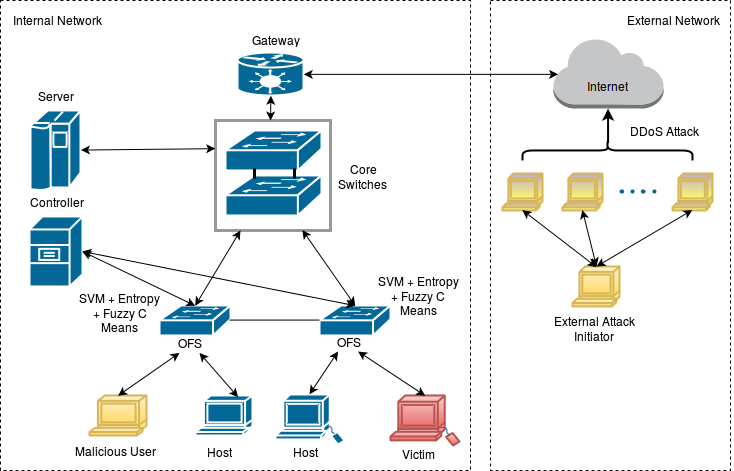
\includegraphics[scale=0.6]{architecture.png}
\caption{System Architecture}
\label{Architecture}
\end{center}
\end{figure}
\newpage

\AddToShipoutPictureBG*{%
\begin{tikzpicture}[overlay,remember picture]
\draw[line width=1.5pt]
    ($ (current page.north west) + (0.7cm,-0.7cm) $)
    rectangle
    ($ (current page.south east) + (-0.7cm,0.7cm) $);
\draw[line width=1.5pt]
    ($ (current page.north west) + (0.9cm,-0.9cm) $)
    rectangle
    ($ (current page.south east) + (-0.9cm,0.9cm) $);
\end{tikzpicture}
}
\chapter{Technical Specification}
\thispagestyle{empty}
\newpage
\section{Technologies Used}
The following technologies will be used in this project :
\begin{enumerate}
\item
SDN Controller:
\begin{itemize}
\item
OpenDaylight :
\newline
At the core of the SDN architecture is the Controller. We will be using the OpenDaylight controller (Beryllium) which will be used to setup our SDN. It is an open source project which is hosted by the Linux Foundation and the goal of this project is to accelerate the adoption of SDN. It is the most widely used SDN controller across various platforms and is an enterprise grade standard controller.

\item
Open Network Operating System (ONOS):
\newline
As an alternative to OpenDaylight, ONOS is another SDN Operating System or Controller. It is especially meant for service providers and designed for performance, scalability and high availability. We will be testing our application using the ONOS controller as well.
\end{itemize}

\item
Mininet :
\newline
Mininet is a network emulator that creates a realistic virtual network, running real kernel, switch and application code, on a single machine within a few seconds. It uses lightweight virtualization to make a single system look like a complete network. Custom topologies can be created in Mininet using Python Scripts. One of Mininet's most powerful features is that it uses SDN. Using the OpenFlow protocol and related tools, you can program switches to do almost anything you want with the packets that enter them. By default if not specified, it uses the ovs-controller. But a remote controller such as OpenDaylight or ONOS can be specified in the mn command to be used.

\item
Open vSwitch :
\newline
Open vSwitch is a production quality, multilayer virtual switch. It leverages OpenFlow and the Open vSwitch Database (OVSDB) management protocol. Using OVS for virtual networking is considered the core element of many data center SDN deployments. Mininet uses Open vSwitch to switch the packets across the interfaces and to make the switches support and operate using the OpenFLow protocol.

\item
LibSVM :
\newline
LibSVM is an open source machine learning library which was developed by National Taiwan University. It is written in C++ along with a C API and is an integrated software for support vector classification. It implements the SMO algorithm for kernelized support vector machines (SVMs), supporting classification and regression. We will be using LIBSVM along with Python.

\item
Python :
\newline
Pyhton is a high-level, interpreted, dynamic programming language. The network topologies in Mininet will be created using Python scripts. Also the SVM and the Entropy implementation will be done from scratch completely in Python. 

\item
Network Monitoring Tool :
\newline
Example: Nagios
\newline
Monitors the entire network and if an entry is made in the log file of the switch then the notification is forwarded to the network administrative team. 
\end{enumerate}
\newpage

\AddToShipoutPictureBG*{%
\begin{tikzpicture}[overlay,remember picture]
\draw[line width=1.5pt]
    ($ (current page.north west) + (0.7cm,-0.7cm) $)
    rectangle
    ($ (current page.south east) + (-0.7cm,0.7cm) $);
\draw[line width=1.5pt]
    ($ (current page.north west) + (0.9cm,-0.9cm) $)
    rectangle
    ($ (current page.south east) + (-0.9cm,0.9cm) $);
\end{tikzpicture}
}
\chapter{Conclusion}
\thispagestyle{empty}
\newpage
The report introduces the problems faced in the Software Defined Networking Environment such as DDoS,
application layer attack, brute force and phishing. As the SDN Controller seperates the Application layer and 
the Data flow plane in the network, it becomes a point of vulnerability for the attackers to target by using 
such attacks.

DDoS attack when targetted on the controller can pose a huge impact on the whole network compromizing the system 
responsible for the Business logic. Thus it is very important to use a mechanism which can detect and mitigate such 
anomaly based attacks, we focus on the prior and not the later part of the mechanism.

There are several methods which can be used for the detection of DDoS such as use of neural networks, chaotic 
systems, filtering algorithms etc. Considering the advantages of Support Vector Machines and Entropy Based Discretization algorithms, we will be using them.

We then procede by stating the product features,user characteristics, system features, interfaces and quality 
attributes like correctness,usability etc. We also provide necessary diagramatic representations like the 
sequence diagram, use case diagram etc.

We then give a description of the system components, system architecture as well as the functioning of the whole
network environment. We also specify two cases of the DDoS attack scenarios namely, internal and external attacks and the method in which we detect the attack using the two proposed algorithmic strategies. After the detection of the attack, the network administrator will be notified by the mechanism and a graphical interface would be provided for the administrator for finding the point of attack.

This project will be a step towards solving the security issues faced right now. This will be a challenging endevour for us as we try to incorporate concepts like networking, machine learning and data mining.  
\newpage

\AddToShipoutPictureBG*{%
\begin{tikzpicture}[overlay,remember picture]
\draw[line width=1.5pt]
    ($ (current page.north west) + (0.7cm,-0.7cm) $)
    rectangle
    ($ (current page.south east) + (-0.7cm,0.7cm) $);
\draw[line width=1.5pt]
    ($ (current page.north west) + (0.9cm,-0.9cm) $)
    rectangle
    ($ (current page.south east) + (-0.9cm,0.9cm) $);
\end{tikzpicture}
}
\SkipTocEntry\chapter{Bibliography}
\thispagestyle{empty}
\newpage
\begingroup
\renewcommand{\chapter}[2]{}
\begin{thebibliography}{9}
\bibitem{BasePaper1}
Diego Kreutz, Fernando M. V. Ramos, Paulo Verissimo, Christian Esteve Rothenberg, Siamak Azodolmolky, Steve Uhlig,
``Software-Defined Networking: A Comprehensive Survey",
Version 2.01,
8 Oct 2014

\bibitem{BasePaper2}
Open Networking Foundation, 
``Software-Defined Networking: The New Norm for Networks",
ONF white paper, 
April 13, 2012

\bibitem{BasePaper3}
Shiva Rowshanrad, Sahar Namvarasl, Vajihe Abdi, Maryam Hajizadeh, Manijeh Keshtgary,
``A survey on SDN, the future of networking",
in Journal of Advanced Computer Science and Technology,
pg 232-248,
2014

\bibitem{BasePaper4}
Rishikesh Sahay, Gregory Blanc, Zonghua Zhang, Herve Debar,
``Towards Autonomic DDoS Mitigation using Software Defined Networking",
Feb 2015,
http://www.internetsociety.org/doc/towards-autonomic-DDoS-mitigation-using-software-defined-networking

\bibitem{BasePaper5}
Seyed Mohammad Mousavi,
``Early Detection of DDoS Attacks in Software Defined Networks Controller",
2014

\bibitem{BasePaper6}
Shunsuke Oshima, Takuo Nakashima, Toshinori Sueyoshi,
``Early DoS/DDoS Detection Method using Short-term Statistics",
Presented at International Conference on Complex, Intelligent and Software Intensive Systems,
2010

\bibitem{BasePaper7} 
Kokila RT, S.Thamarai Selvi, Kannan Govindarajan,
``DDoS Detection and Analysis in SDN-based Environment Using Support Vector Machine Classifier",
presented at Sixth International Conference on Advanced Computing(ICoAC),
2014,

\bibitem{BasePaper8}
Xue Li, Dongming Yuan, Hefei Hu, Jing Ran, Shulan Li, 
``DDoS detection in SDN switches using support vector machine classifier",
in Joint International Mechanical, Electronic and Information Technology Conference, 
2015

\bibitem{BasePaper9} 
Rui Wang, Zhiping Jia∗, Lei Ju,
``An Entropy-Based Distributed DDoS Detection Mechanism in Software-Defined Networking",
in IEEE Trustcom/BigDataSE/ISPA,
DOI 10.1109/Trustcom.2015.389,
2015

\bibitem{BasePaper10}
T.Subbulakshmi, Dr. S. Mercy Shalinie, V.GanapathiSubramanian, K.BalaKrishnan, D. AnandKumar, K.Kannathal,
``Detection of DDoS Attacks using Enhanced Support Vector Machines with Real Time Generated Dataset",
in IEEE-ICoAC, 
2011

\bibitem{BasePaper11}
I Gde Dharma N., M. Fiqri Muthohar, Alvin Prayuda J. D., Priagung K., Deokjai Choi,
``Time-based DDoS Detection and Mitigation for SDN Controller",
Presented at APNOMS,
2015

\bibitem{BasePaper12}
Shibo Luo, Jun Wu, Jianhua Li,
``A Defense Mechanism for Distributed Denial of Service Attack in Software-Defined Networks",
Presented at Ninth International Conference on Frontier of Computer Science and Technology,
2015

\bibitem{BasePaper13}
K. Giotis, C. Argyropoulos, G. Androulidakis, D. Kalogeras, V. Maglaris,
``Combining OpenFlow and sFlow for an effective and scalable anomaly detection and mitigation mechanism on SDN environments",
2013, 
http://dx.doi.org/10.1016/j.bjp.2013.10.014

\bibitem{BasePaper14}
Seyed Mohammad Mousavi, Marc St-Hilaire,
``Early Detection of DDoS Attacks against SDN Controllers",
Presented at International Conference on Computing, Networking and Communications, Communications and Information Security
Symposium,
2015

\bibitem{BasePaper15}
P. K. Agrawal, B. B. Gupta, Satbir Jain,
``SVM Based scheme for Predicting Number of Zombies in a DDoS Attack",
Presented at European Intelligence and Security Informatics Conference,
2011

\bibitem{BasePaper16}
A. Ramamoorthi, T. Subbulakshmi, Dr. S. Mercy Shalinie,
``Real Time Detection and Classification of DDoS Attacks using Enhanced SVM with String Kernels",
in IEEE-International Conference on Recent Trends in Information Technology,
ICRTIT 2011,
June 2011

\bibitem{BasePaper17}
Ingo Steinwart, Andreas Christmann,
``Support Vector Machines",
Springer, 
2008

\bibitem{BasePaper18}
Alexander Gelbukh, Félix Castro Espinoza, Sofía N. Galicia-Haro,
``Nature-Inspired Computation and Machine Learning",
Springer,
2014
\end{thebibliography}
\endgroup
\newpage

\AddToShipoutPictureBG*{%
\begin{tikzpicture}[overlay,remember picture]
\draw[line width=1.5pt]
    ($ (current page.north west) + (0.7cm,-0.7cm) $)
    rectangle
    ($ (current page.south east) + (-0.7cm,0.7cm) $);
\draw[line width=1.5pt]
    ($ (current page.north west) + (0.9cm,-0.9cm) $)
    rectangle
    ($ (current page.south east) + (-0.9cm,0.9cm) $);
\end{tikzpicture}
}
\SkipTocEntry\chapter{Appendix - A}
\thispagestyle{empty}
\newpage
\SkipTocEntry\section{Appendix A.1}
\SkipTocEntry\subsection{IDEA Matrix}
\begin{table}[h]
\caption{IDEA Matrix}

\begin{center}
\begin{tabular}{|>{\bf}M{2.5cm}||>{\bf}M{2.5cm}||>{\bf}M{2.5cm}||>{\bf}M{2.5cm}|}
\hline
\rowcolor{lightgray}
I & D & E & A \\ \hline
\normalfont{Innovative} & \normalfont{Detect}  & \normalfont{Evaluate} & \normalfont{Associate} \\ \hline
\normalfont{Increase} & \normalfont{Decrease}  & \normalfont{Effective} & \normalfont{Acquire} \\ \hline
\normalfont{Investment} & \normalfont{Depict}  & \normalfont{Enhance} & \normalfont{Analyse} \\ \hline
\end{tabular}
\end{center}
\end{table}

\begin{center}
\begin{tabular}{|m{2cm}|m{7cm}|}
\hline
Innovative & Up till now, DDoS detection systems uses a single mechanism for its working. Here, the system will be using two mechanisms i.e. support vector machine and entropy based discretization simultaneously which is \textbf{innovative}. \\

&\\

Increase & As the system will be using support vector machine and entropy based discretization, efficiency of the system will \textbf{increase}. \\

&\\

Investment & As the system contains Software components only. So, \textbf{zero investment} is required to implement the system in already deployed software defined network. \\

\hline
\end{tabular}
\end{center}

\vspace*{1cm}
\begin{center}
\begin{tabular}{|m{2cm}|m{7cm}|}
\hline

Detect & The system will \textbf{detect} DDoS attack and raise notification to the network administrator team. \\

&\\

Decrease & The DDoS detection algorithm will \textbf{decrease} the possibility of false positive attack detection. \\

&\\

Depict & The system will \textbf{depict} appropriately whether the network traffic is normal or attack traffic. \\

\hline
\end{tabular}
\end{center}

\newpage
\begin{center}
\begin{tabular}{|m{2cm}|m{7cm}|}
\hline

Evaluate & An important part of the implementation is the \textbf{evaluation} of the rate of flow of packets per unit time. \\

&\\

Effective & The system analyses the traffic and detects the attack at runtime thus, increasing the \textbf{effectiveness}. \\

&\\

Enhance & The accuracy of the system will be \textbf{enhanced} by using an environment - specific training dataset for SVM. \\

\hline
\end{tabular}
\end{center}

\vspace*{1cm}
\begin{center}
\begin{tabular}{|m{2cm}|m{7cm}|}
\hline

Associate & The project is a step towards \textbf{association} and integration of next generation networking with advanced computing concepts like Machine Learning and Data Mining. \\

&\\

Acquire & The flow table containing the flow entries along with the information of the count of the packets is \textbf{acquired} from the SDN switches. \\

&\\

Analyse & The system will \textbf{analyse} the data acquired from the switches to perform the intended task of detecting the DDoS attack. \\

\hline
\end{tabular}
\end{center}

\newpage
\SkipTocEntry\section{Appendix A.2}
\SkipTocEntry\subsection{Mathematical Model}
{\setlength{\mathindent}{0cm}
\begin{equation}
S = \lbrace \lbrace I \rbrace ,\lbrace P \rbrace,\lbrace O \rbrace \rbrace
\end{equation}

\noindent
where,\\
$I =$ Input set,\\
$P = \lbrace P_{EBD}, P_{SVM} \rbrace$ Processing set, \\
$O =$ Output set

\SkipTocEntry\subsection{Input:}
{\setlength{\mathindent}{0cm}
\begin{equation}
I = \lbrace N \rbrace
\end{equation}

\noindent
where,\\
$N = \lbrace $ Network Statistics $ \rbrace $, \\
$F =\lbrace F_{i} \mid F_{i} \in T , \forall i$ $ F_{i} =$ Individual entry $ \rbrace$, \\
$T = \lbrace $ Flow Table $ \rbrace$, \\
$F \subseteq N$

\SkipTocEntry\subsection{Input for EBD:}

{\setlength{\mathindent}{0cm}
\begin{equation}
I_{EBD} = \lbrace U_{i} \mid U_{i} = ($ Source Address, Destination Address, Port no., Count$),  $ $ U_{i}  \subset F_{i} \rbrace
\end{equation}

\SkipTocEntry\subsection{Input for SVM:}

{\setlength{\mathindent}{0cm}
\begin{equation}
I_{SVM} = \lbrace V_{i} \mid V_{i} = ($ Source Address, Destination Address, Port no., Time, Protocol, Count$),  $ $ V_{i}  \subset F_{i} \rbrace
\end{equation}

\SkipTocEntry\subsection{Processing:}
$P_{EBD} $ $ (I_{EBD},$ $O_{EBD})$\\
$\lbrace$

\begin{enumerate}

\item 
{\setlength{\mathindent}{0cm}}
\begin{equation}
P_{i} = \frac{C_{i}}{N}
\end{equation}
where, \\ $c =$ counter, \\ $N = \sum_{i=0}^{n} C_{i}$, \\ $n =$ no. of entries.

\item 
{\setlength{\mathindent}{0cm}}
\begin{equation}
\varepsilon = \sum_{i=0}^{n} - P_{i} log P_{i}
\end{equation}

\newpage
\item 
\begin{equation}
(\lambda < \varepsilon) \rightarrow (\beta = 0)
\end{equation}
\begin{equation}
(\lambda > \varepsilon) \rightarrow (\beta = 1)
\end{equation}

\item  
\begin{equation}
O_{EBD} = \lbrace \beta \mid \beta \in (0,1) \rbrace
\end{equation}

\end{enumerate}

$\rbrace$
\\

\noindent
$P_{SVM} $ $ (I_{SVM},$ $O_{SVM})$\\
$\lbrace$
\indent
Here, \\
\indent $\gamma$ , $c$, $x$, $x_{1}$, $x_{2}$, $b$ and $\overline{\omega}$ are constants.\\
\indent These values are calculated from Training Phase.\\
\indent Training of SVM is based on dataset used.


\begin{enumerate}

\item 
\begin{equation}
RBF = e^{-\gamma(\mid x_{1}-x_{2} \mid)+c}
\end{equation}
where, \\ $\gamma =$ width of boundries of hyperplane, \\ $c =$ soft margin parameter, \\ $x_{1}, $ $x_{2} =$ support vectors.


\item
\begin{equation}
y = \overline{\omega} * x + b
\end{equation}
where, \\ $x =$ support vector, \\ $b =$ boundary width, \\ $\overline{\omega} =$ libsvm.w().

\item
\begin{equation}
(y \leq -1) \rightarrow (\alpha = 1)
\end{equation}
\begin{equation}
(y \geq 1) \rightarrow (\alpha = 0)
\end{equation}

\item
\begin{equation}
O_{SVM} = \lbrace \alpha \mid \alpha \in (0, 1) \rbrace
\end{equation}

\end{enumerate}

$\\ \rbrace$

\SkipTocEntry\subsection{Output:}

\begin{equation}
O_{EBD} = \lbrace z \mid \exists z, z \in \beta \rbrace
\end{equation}
\begin{equation}
O_{SVM} = \lbrace x \mid \exists x, x \in \alpha \rbrace
\end{equation}
\begin{equation}
O_{system} = \lbrace O_{EBD} \cup O_{SVM} \rbrace
\end{equation}

\SkipTocEntry\subsection{Feasibility Study}
To check the feasibility of Entropy Based Discretization and Support Vector Machine:
\newline Since, the problem we solve is essentially a decision problem, it is very essential to analyse the running time of the system. The two strategies used in the system are SVM and Entropy Based Discretization. It is well known that EBD takes O(n) running time thus is in P.\\
\newline
Now, we will find the computational complexity for Support Vector Machines:\\
For a training dataset D=\{$x_i$,$y_i$\} where, $x_i$ $\in$ $\Re$ and $y_i$ $\in$ \{+1,-1\}.\\
The Support Vector Machine classifies with seperating hyperplane given by:\\

\begin{equation}
D(x)=w^Tx+b
\end{equation}

The above equation is obtained by:
\begin{equation}
L=\frac{1}{2} \emph{w}^2 - \sum_{}^{} \zeta_i
\end{equation}

s.t. $y_i$($w^T$ $x_i$ + b) $\geq$ 1 - $\zeta_i$, $\zeta_i$ $>$ 0 for i=1,2,...,m \\
\newline The problem is equivalent to the problem:\\
\begin{equation}
Max L(\alpha)= \sum_{i=1}^{M} \alpha_i - \frac{1}{2} \sum_{i=1}^{m}\sum_{j=1}^{m} y_iy_j\alpha_i\alpha_jk(x_i,y_j)
\end{equation}

where k($x_1$,$y_1$) is the Mercer's Kernel which is used for the 
Dimensional reduction.\\
\newline We will use the following four steps to prove the complexity of the SVM problem:
\begin{enumerate}
\item
Denote the problem as \textbf{$\pi$} and justify that it is in NP.
\item
Selecting a known problem \textbf{$\pi$'} which is in NP.
\item
Construct a tranformation function from $\pi$' to $\pi$.
\item
Prove that the transformation function is polynomial.
\end{enumerate}
\begin{itemize}
\newpage
\item
\textbf{The SVM Problem ($\pi$)}
\newline For a set of kernels A=\{$k_1,k_2,...,k_n$\} the objective function can be written as:\\

\begin{equation}
C(A')=	\Big[\sum_{k \in A'}^{}\Big(\frac{1}{q}\Big[\sum_{i=1}^{m} \alpha_i - \frac{1}{2q^2} \sum_{i=1}^{m}\sum_{j=1}^{m}y_iy_jk(x_i,x_j)\alpha_i\alpha_j\Big]\Big)^2- B\Big]^2
\end{equation}	
\newline 

Where, we have to find a subset A' $\subseteq$ A of size q to minimize the cost. The cost function is used for reaching a bound B using set of Kernels, dataset and the Support Vectors.\\
\item
\textbf{SVM is in NP}
\newline To justify that SVM is in NP, we have to show that any instance of the problem can be guessed and verified to solve or not in polynomial time.\\
Let there be a function, that accepts q which returns random indices of q from the set of kernels and computes the most optimum solution A'. As the set of Lagrange Multipliers, dataset, q and Bound is known beforehand, the kernel evaluations are the only states.  These kernel evaluations are merely dot products among the directional vectors. The evaluation is polynomial and thus the instances A' can easily be generated and verified. Hence, we can say that SVM is in NP.
\item
\textbf{Selecting a known NP-Complete Problem ($\pi$')}
\newline The known problem selected is the subset problem which is as defined,\\
Given a set A, a size s(a) for each a $\in$ A and an integer B. Is there an A' $\subseteq$ A such that the sum of the sizes of the elements in is exactly B?\\
\item
\textbf{Transformation function $\mathcal{F}$ from $\pi$' to $\pi$}
\newline The transformation function $\mathcal{F}$ should map every instance (\emph{I}) such that every instance of "yes" in $\pi$ should map to the corresponding instance (\emph{I'}) in $\pi$'.\\
First, A stands for set of kernels: A=\{$A_1,A_2,...,A_n$\} \\
To compute B the following procedure should be followed: \\
\begin{enumerate}
\item
Solve SVM for all k $\in$ A with dataset D.
\item
Use the kernel $k^*$ and the dataset D to find the most optimal solution for SVM denoted by $M^* = (V^*,k^*)$
\item 
Now, B can be calculated by:- 
\begin{equation}
B = \Big[\sum_{i=1}^{m} \alpha_i - \frac{1}{2}\sum_{i=1}^{m}\sum_{j=1}^{m}y_iy_jk^*(x_i,x_j)\alpha_i,\alpha_j\Big]^2
\end{equation} 
\item
Finally we have to calculate the size function s(a)=s(k $\in$ A) which can be done by the formula:- \\
\begin{equation}
s(k) = \Big[\big(\frac{1}{q}\sum_{i=1}^{m}\alpha_i - \frac{1}{2q^2}\sum_{i=1}^{m}\sum_{j=1}^{m}y_iy_jk(x_i,x_j)\alpha_i\alpha_j\Big)\Big]^2
\end{equation}
Where, s(k) is the value of the objective function. 
\end{enumerate} 
Now, we know that $\sum_{k \in A}^{}s(k)=B$ when $k^*(x_i,x_j)=\frac{1}{q^2}\sum_{k \in A'}^{},(k_i,k_j)$ \\
This can be written in the form: \\
\begin{equation}
\Big[\sum_{k \in A'}^{}\Big(\frac{1}{q}\sum_{i=1}^{m}\alpha_i - \frac{1}{2q^2}\sum_{i=1}^{m}\sum_{j=1}^{m}y_iy_jk(x_i,x_j)\alpha_i\alpha_j\Big) \Big]^2 = \Big[\sum_{i=1}^{m} \alpha_i - \frac{1}{2}\sum_{i=1}^{m}\sum_{j=1}^{m}y_iy_jk^*(x_i,x_j)\alpha_i\alpha_j\Big]^2
\end{equation}
Taking squared-root and using summation property, \\
\begin{equation}
\sum_{k \in A'}\Big(\frac{1}{q}\sum_{i=1}^{m}\alpha_i\Big)+\sum_{k \in A'}^{}\Big[-\frac{1}{2q^2}\sum_{i=1}^{m}\sum_{j=1}^{m}y_iy_jk(x_i,x_j)\alpha_i\alpha_j\Big] = \sum_{i=1}^{m}\alpha_i-\frac{1}{2}\sum_{i=1}^{m}\sum_{j=1}^{m}y_iy_jk^*(x_i,x_j)\alpha_i\alpha_j
\end{equation}
Simplifying the equation,
\begin{equation}
\sum_{k \in A'}\Big[\frac{1}{q^2}\sum_{i=1}^{m}\sum_{j=1}^{m}y_iy_jk(x_i,x_j)\alpha_i\alpha_j\Big] = \sum_{i=1}^{m}\sum_{j=1}^{m}y_iy_jk^*(x_i,x_j)\alpha_i\alpha_j
\end{equation}
Substituting $\Delta_{i,j}$ = $y_iy_j\alpha_i\alpha_j$ for simplification purpose \\
\begin{equation}
\sum_{k \in A'}\Big[\frac{1}{q^2}\sum_{i=1}^{m}\sum_{j=1}^{m}\Delta_{i,j}k(x_i,x_j)\Big] = \sum_{i=1}^{m}\sum_{j=1}^{m}\Delta_{i,j}k^*(x_i,x_j)
\end{equation}
Cancelling common terms,
\begin{equation}
\frac{1}{q^2}\sum_{k \in A'}{}k(x_i,x_j)=k^*(x_i,x_j)
\end{equation}
Thus, 
\begin{equation}
\sum_{k \in A'}s(k) = B \leftrightarrow k^*(x_i,x_j) = \frac{1}{q^2}\sum_{k \in A'}k(x_i,x_j)
\end{equation}
This implies that the transformed subset problem is equivalent to SVM classification using an optimum kernel. Thus, for every instance of (\emph{I')} if the answer is "yes" the answer can be mapped for the instance  of (\emph{I}). \\
\item
\textbf{$\mathcal{F}$ is a polynomial Transformation}
\newline The last part is to prove that the $\mathcal{F}$ is polynomial. The most expensive step is to find the Boundary (B) in the training phase.\\
This problem of training is a quadratic problem(QP). This problem can be seen as a convex problem. There are methods like Ellipsoids to solve it in polynomial time. 
It is also known that QP can be solved in O($m^3$), for  SVM ``m'' is the number of input vectors. Therefore, $\mathcal{F}$ is a polynomial transformation. \\
\newline Thus, SVM is a NP-Complete.\\
Also Entropy Based Discretization is in P.\\
By Cook's theorem, P $\in$ NP therefore, the proposed algorithmic strategy is NP-Complete.  

\end{itemize}

\newpage
\SkipTocEntry\section{Appendix A.3}
\SkipTocEntry\subsection{Distributed Computation}
The controller in an Software Defined Network is the centralized entity, which is responsible for the interfacing between Application layer and the underlying network hardware. Since, the controller imposes the application logic onto the datapath of the SDN. This requires a lot of computation. \\

	Furthermore, during the scenario of a DDoS attack there is an excruciating load on the network and especially the SDN controller.	Thus, is unwise to run an application on top of the controller as it can cause an overhead on the system. We exploit the dormant processing power of the SDN switches to our advantage by using them as computational nodes. Our DDoS detection mechanism will work on the switches distributed throughout the network. \\

Each switch will scan its underlying traffic. The advantages of this are twofold firstly, there will not be an overhead on the remaining network and secondly, it will be easier for the network administrator for finding the origin of the DDoS attack vastly reducing the cost and effort for the recovery. \\

Thus, we divide the whole network traffic statistics into several concurrent switches for the computation making it a divide and conquer strategy.

\SkipTocEntry\subsection{Functional Dependancies}
There are mainly four Functions in the system namely,
\begin{enumerate}
\item
A function which will continuously send the formatted traffic statistics which can be accepted by the Support Vector Machine and Entropy Based Descretization mechanism.
\item
A Funtion for the support vector machine classifier which will classify the traffic into normal or attack traffic and update the log files if attack traffic is detected.
\item
A Function for the Entropy based discretization mechanism which will compare the flow of traffic with the threshold value and update the log files if the rate of flow of packets exceeds the threshold.
\item
A Function which will monitor the log files to check whether there is an attack scenario or not.
\end{enumerate}
The SVM and Entropy Based Mechanism depend on the real-time input of the flow table entries, the function responsible for monitoring is dependent on the SVM and Entropy mechanism. Thus, there is a one-many-one mapping between this function.
\begin{center}
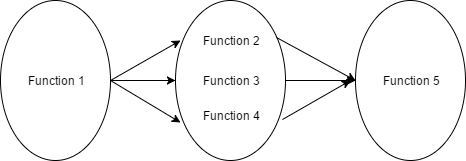
\includegraphics[scale=0.5]{functionalDependency.png}
\end{center}
\newpage

\AddToShipoutPictureBG*{%
\begin{tikzpicture}[overlay,remember picture]
\draw[line width=1.5pt]
    ($ (current page.north west) + (0.7cm,-0.7cm) $)
    rectangle
    ($ (current page.south east) + (-0.7cm,0.7cm) $);
\draw[line width=1.5pt]
    ($ (current page.north west) + (0.9cm,-0.9cm) $)
    rectangle
    ($ (current page.south east) + (-0.9cm,0.9cm) $);
\end{tikzpicture}
}
\SkipTocEntry\chapter{Appendix - B}
\thispagestyle{empty}
\newpage

\SkipTocEntry\section{Appendix B.1}
\SkipTocEntry\subsection{Test Cases :}
\begin{center}
\begin{tabular}{|p{1cm}|p{3cm}|p{3cm}|p{3.5cm}|}
\hline 
 \textbf{Id} & \textbf{Description} & \textbf{Scenario} & \textbf{Expected Output} \\ 
\hline 
 1 & Time span between attack detection and alert generation & Attack has occured & Instantaneous alert generation\\
 \hline
 2 & Normal Network Traffic, Log file not altered and attack is not detected & SDN functioning in normal mode & Alert not generated\\ 
\hline 
\end{tabular} 
\end{center}

\SkipTocEntry\subsection{Scenario: Attack Traffic}
\begin{center}
\begin{tabular}{|p{1cm}|p{3cm}|p{3cm}|p{3.5cm}|}
\hline 
 \textbf{Id} & \textbf{Description} & \textbf{Input} & \textbf{Expected Output} \\ 
\hline 
 1 & Simple DoS attack & Large no. of same type of packets & Attack detected\\
 \hline
 2 & UDP flood attack & Large no. of UDP packets & Attack detected\\ 
 \hline
 3 & TCP-SYN attack & Large no. of TCP-SYN request & Attack detected\\
 \hline
 4 & ICMP or Ping flood attack & Large no. of ICMP ECHO request & Attack detected\\
 \hline
 5 & HTTP flood attack on web server & Large no. of HTTP request & Attack detected\\
 \hline
 6 & Varying DDoS attack bandwidth & Large no. of packets & DDoS attack should be detected only when bandwidth exceeds normal threshold traffic. \\
\hline 
\end{tabular} 
\end{center}

\SkipTocEntry\subsection{Scenario: Normal Traffic}
\begin{center}
\begin{tabular}{|p{1cm}|p{3cm}|p{3cm}|p{3.5cm}|}
\hline 
 \textbf{Id} & \textbf{Description} & \textbf{Input} & \textbf{Expected Output} \\ 
\hline 
 1 & Normal traffic on web server & Normal traffic of HTTP request & Attack not detected\\
 \hline
 2 & Normal Ping request-reply & ICMP packets & Attack not detected\\ 
 \hline
 3 & Normal file transfer & FTP packets & Attack not detected\\
 \hline
 4 & Video buffering & UDP packets & Attack not detected\\
 \hline
 5 & Web browsing & HTTP or TCP packets & Attack not detected\\
\hline 
\end{tabular} 
\end{center}
\newpage

\AddToShipoutPictureBG*{%
\begin{tikzpicture}[overlay,remember picture]
\draw[line width=1.5pt]
    ($ (current page.north west) + (0.7cm,-0.7cm) $)
    rectangle
    ($ (current page.south east) + (-0.7cm,0.7cm) $);
\draw[line width=1.5pt]
    ($ (current page.north west) + (0.9cm,-0.9cm) $)
    rectangle
    ($ (current page.south east) + (-0.9cm,0.9cm) $);
\end{tikzpicture}
}
\SkipTocEntry\chapter{Appendix - C}
\thispagestyle{empty}
\newpage

\SkipTocEntry\section{Appendix C.1}
\SkipTocEntry\subsection{Milestones}
\begin{center}
\begin{tabular}{ |p{5cm}|p{3cm}|p{3cm}|p{1.5cm}| } 
 \hline
 \textbf{Name} & \textbf{Start Date} & \textbf{Due Date} & \textbf{Priority} \\ \hline
  Domain Selection & $15^{th}$ June 2016 & $30^{th}$ June 2016 & High \\ \hline
  Topic Finalization & $1^{st}$ July 2016 & $10^{th}$ July 2016 & High \\ \hline
  Feasibility Study and Market Potential Analysis & $11^{th}$ July 2016 & $25^{th}$ July 2016 & High \\ \hline
  Abstract Submission & - & $26^{th}$ July 2016 & Medium \\ \hline
  System Architecture Design & $1^{st}$ Aug 2016 & $20^{th}$ Aug 2016 & High \\ \hline    
  Discussion about Platform issues & $21^{st}$ Aug 2016 & $30^{th}$ Aug 2016 & High \\ \hline
  Preparing Synopsis & $1^{st}$ Sept 2016 & $20^{th}$ sept 2016 & High \\ \hline
  Project Report Submission for Stage I & - & $5^{th}$ Oct 2016 & Medium \\ \hline
  Discussion about Platform Selection & $1^{st}$ Dec. 2016 & $15^{th}$ Dec. 2016 & High \\ \hline
  System Design and Coding & $20^{th}$ Dec. 2016 & $15^{th}$ Feb. 2017 & High \\ \hline
  Testing & $16^{th}$ Feb. 2016 & $15^{th}$ Macrh 2016 & High \\ \hline
  Final Report Preparation & - & $15^{th}$ April 2016 & High \\ \hline
\end{tabular}
\end{center}
\end{document}